\chapter{Objetivos y metodología de trabajo}

\section{Objetivo General}

    Desarrollar un modelo de superresolución para mejorar la resolución espacial de imágenes Sentinel-2 de 10 y 20 metros a 2.5 metros, utilizando redes neuronales convolucionales y técnicas de fusión multiespectral.


\section{Objetivos Específicos}

\begin{enumerate}
    \item \textbf{Explorar e implementar técnicas avanzadas de fusión de imágenes:} Mejorar la resolución espacial y espectral de datos multiespectrales de Sentinel-2, preservando las características originales.
    \item \textbf{Desarrollar un modelo de fusión de imágenes basado en aprendizaje profundo:} Crear un modelo que combine datos multiespectrales para generar imágenes de mayor resolución espacial manteniendo la integridad espectral.
    \item \textbf{Aplicar el Protocolo de Wald para la validación:} Utilizar el Protocolo de Wald para asegurar que las imágenes super-resueltas mantengan consistencia con las imágenes originales en términos de propiedades espaciales y espectrales.
    \item \textbf{Evaluar el rendimiento del modelo propuesto:} Analizar cómo la superresolución mejora la detección de inundaciones mediante índices de humedad y métricas de rendimiento.
\end{enumerate}

\section{Metodología de trabajo}

    Este trabajo emplea un enfoque de fusión en dos etapas: \textbf{Fusión x2} y \textbf{Fusión x4}, para mejorar la resolución espacial de imágenes satelitales Sentinel-2. Estas etapas permiten una transición progresiva desde resoluciones originales de \textit{10} y \textit{20 metros} a una resolución final de \textit{2.5 metros}, manteniendo la integridad espectral y espacial de los datos.

    Las bandas multiespectrales, con resoluciones originales diferentes, se procesan de manera diferenciada en cada etapa de fusión. Este enfoque asegura que la metodología capture y preserve tanto los detalles espaciales como las características espectrales del entorno observado.


    \subsection{Obtención y procesamiento de los datos}

        Para el desarrollo de este proyecto, se utiliza el conjunto de datos \textit{CloudSEN12} de \textcite{aybar2024cloudsen12+}, un dataset global diseñado para la comprensión semántica de nubes y sombras de nubes en imágenes Sentinel-2. Este conjunto es accesible a través de Hugging Face, siguiendo los pasos indicados en este \href{https://colab.research.google.com/drive/10QqUk-4pP6lZHj1I9GfMpzDY-cd0Fdza?usp=sharing}{\textit{Colab} público} e incluye un total de \textit{49,400} imágenes en formato \textit{Level-1C} (TOA), de las cuales se seleccionan \textit{10,440} imágenes libres de nubes.

        \begin{figure}[H] 
            \caption{\doublespacing \\ \textit{Área de aplicación: ciudad de Valencia}} 
            \centering
            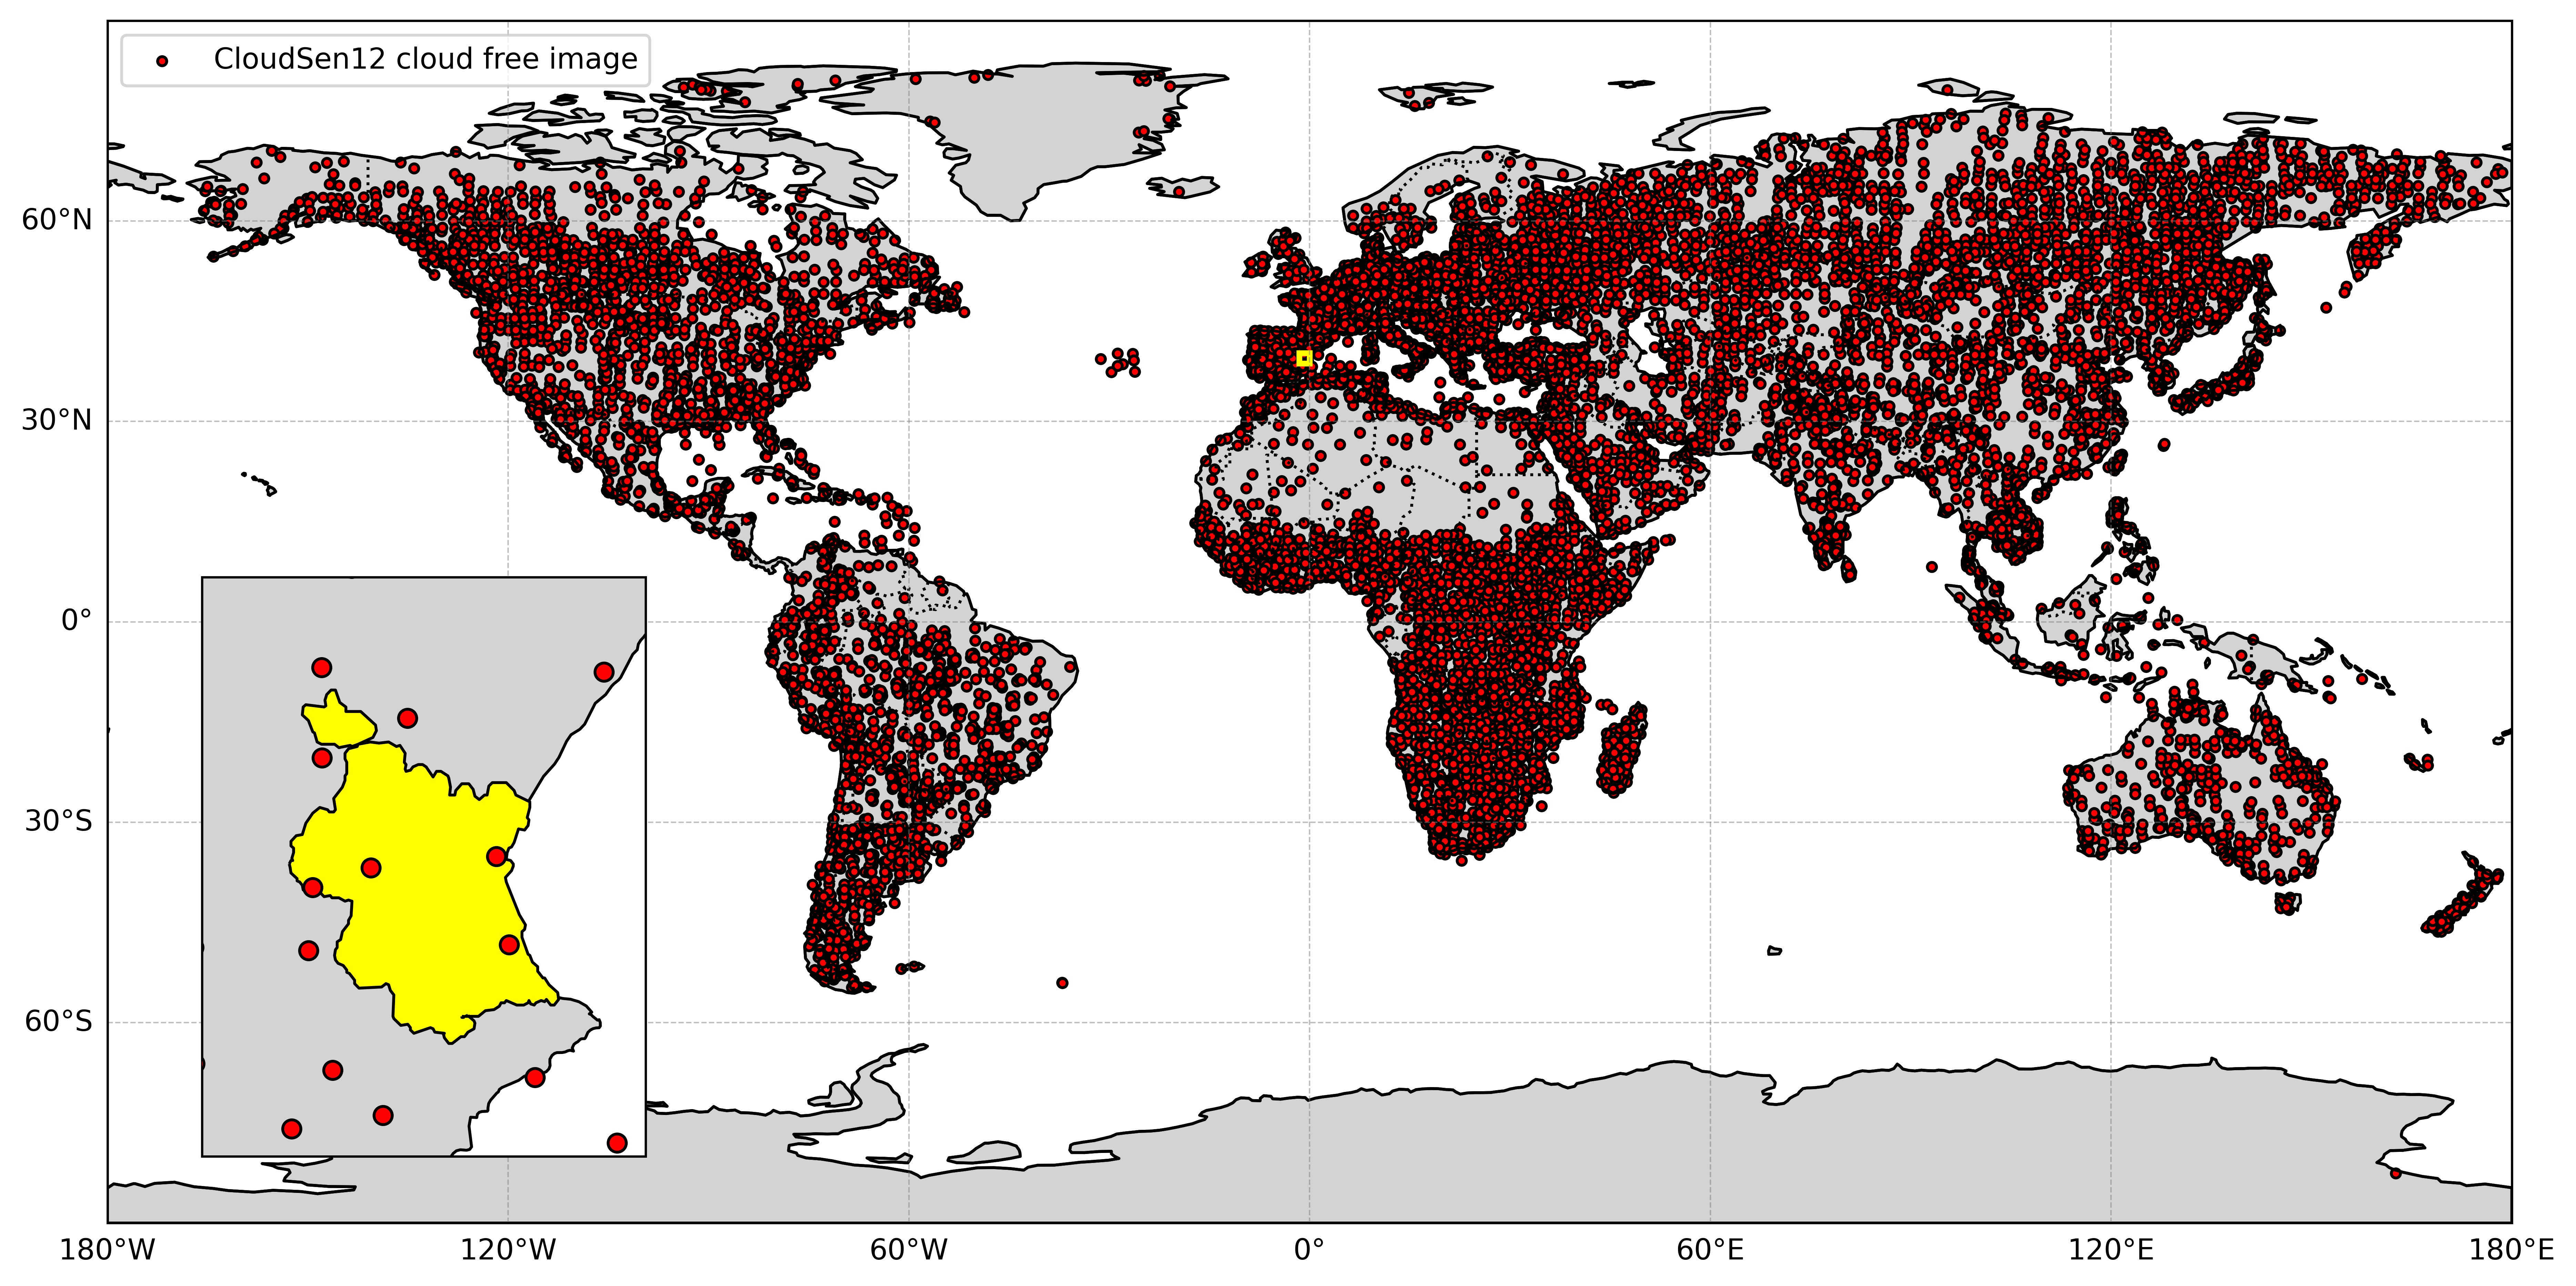
\includegraphics[width=1\linewidth]{images/mapa_valencia.png}
            \begin{justify}
                \textit{Nota.} Se muestran imágenes sin nubes del proyecto CloudSEN12 en zonas de alta heterogeneidad espectral que enriquecen el modelo, destacando la ciudad de Valencia como área de aplicación para evaluar la mejora en la detección de inundaciones mediante superresolución ante su reciente vulnerabilidad a eventos extremos como un DANA (octubre, 2024). Elaboración propia.
            \end{justify}                    
            \label{fig:mapa_valencia}
        \end{figure}
        
        \subsubsection{Preprocesamiento de los datos}

            Las imágenes, que contienen bandas de 10 y 20 metros, provienen del conjunto de datos \textit{CloudSEN12}, donde fueron descargadas con una resolución uniforme de 10 metros, utilizando el método de remuestreo de vecino más cercano (\textit{nearest neighbor}) desde Google Earth Engine (\textit{GEE}). Este proceso asegura la consistencia espacial necesaria para la integración multiespectral.

        \subsubsection{Imágenes sin nubes}

            El uso de imágenes libres de nubes garantiza que el modelo analice exclusivamente las características reales de la superficie terrestre. Esto elimina la necesidad de reconstrucciones adicionales, comunes en áreas con nubes, y mejora la fiabilidad del análisis multiespectral, como señala \textcite{li2023transformer}.

        \subsubsection{Heterogeneidad espectral}

            La selección de regiones con alta diversidad espectral, evitando áreas homogéneas como océanos y zonas polares, enriquece el conjunto de datos. Este enfoque fortalece la capacidad del modelo para capturar una mayor variedad de patrones espectrales, siguiendo recomendaciones de estudios como \textcite{jiao2023integrated}.

        \subsubsection{Selección del área de aplicación}

            La ciudad de Valencia se selecciona como área de aplicación para evaluar cómo la superresolución mejora la detección de inundaciones. Esta región, vulnerable a eventos extremos como un DANA (octubre, 2024), representa un escenario adecuado para analizar el impacto de esta metodología en tareas prácticas de monitoreo y gestión de desastres.


    \subsection{Metodología general para la fusión}

        En ambas etapas de fusión se siguen procedimientos similares en cuanto a la preparación de datos, el filtrado en el dominio de Fourier y el uso de mecanismos de atención mediante SPAN (\textit{Self-parameterized Attention Network}). A continuación, se describen los elementos clave de la metodología aplicada en el proceso.


        \subsubsection{Preparación de datos}

            La preparación de datos garantiza la alineación y normalización de las bandas de diferentes resoluciones, facilitando su integración como entrada en el modelo. La normalización se realiza dividiendo los valores de los píxeles entre \textit{10,000}, ajustando el rango de datos y mejorando la estabilidad durante el entrenamiento.

            Durante el entrenamiento, para fomentar la generalización y prevenir el \textit{overfitting}, se aplica un muestreo aleatorio que selecciona porciones distintas de las imágenes en cada época. Los lotes de datos se reorganizan en cada iteración, evitando que el modelo dependa de un orden específico y fortaleciendo su capacidad de generalización.
            
            En la fase de prueba, se extrae una porción central de cada imagen y los datos se presentan en un orden fijo, garantizando evaluaciones consistentes y reproducibles, libres de la variabilidad introducida por el muestreo aleatorio.

            \paragraph{Bandas de referencia}

                Las bandas de 10 metros, correspondientes a las regiones espectrales del espectro visible (RGB) y NIR (bandas 2, 3, 4 y 8), sirven como referencia para enriquecer la información espacial y espectral en ambas etapas de fusión. Según el requerimiento de cada etapa, estas bandas se usan en su resolución original o se escalan para integrarse con otras bandas.


            \paragraph{Bandas ajustadas}

                Las bandas de 20 metros (bandas 5, 6, 7, 8A, 11 y 12) aportan información clave del borde rojo y el infrarrojo de onda corta. Su resolución viene ajustada a 10 metros mediante interpolación bilineal con antialiasing, asegurando una integración precisa en cada etapa de fusión.

        \subsubsection{Filtrado en el dominio de Fourier}

            Para separar los componentes de alta y baja frecuencia y optimizar el procesamiento de la imagen, se emplea un filtro en el dominio de Fourier. Se utiliza un filtro Butterworth de orden 6, ajustado según el factor de escala específico de cada etapa, para definir un radio de frecuencia en la máscara de paso bajo. Este procedimiento preserva los detalles esenciales mientras se atenúan las frecuencias no deseadas, garantizando una representación equilibrada entre la estructura global y los detalles finos.

        \subsubsection{Arquitectura del modelo y SPAN}

            El modelo de super-resolución se basa en una arquitectura de red neuronal convolucional que incorpora bloques de atención auto-parametrizados SPAB (\textit{Self-parameterized Attention Blocks}). Estos bloques permiten al modelo enfocarse en áreas de la imagen que requieren mayor detalle, mejorando la calidad de la imagen fusionada.

            Dentro de cada SPAB, se utilizan módulos convolucionales personalizados denominados \texttt{Conv3XC}. Estos módulos están diseñados para capturar características complejas de la imagen mediante una serie de operaciones convolucionales y conexiones residuales. La estructura del bloque \texttt{Conv3XC} es la siguiente:

            \begin{enumerate}
                \item \textbf{Primera convolución}: Convierte las características de entrada a un espacio intermedio de mayor dimensionalidad.
                \item \textbf{Segunda convolución}: Aplica una convolución con un kernel de tamaño 3x3 para capturar patrones locales y detalles finos.
                \item \textbf{Tercera convolución}: Reduce la dimensionalidad de las características al número deseado de canales de salida.
                \item \textbf{Conexión residual}: Una convolución 1x1 que conecta directamente la entrada con la salida del bloque, facilitando el flujo de gradientes y mejorando la capacidad de aprendizaje.
            \end{enumerate}

            Estas operaciones permiten al modelo aprender representaciones profundas y detalladas de las imágenes, capturando tanto la información global como los detalles locales. Las activaciones utilizadas incluyen funciones como \textit{SiLU} y \textit{Leaky ReLU}, que contribuyen a una mejor representación de las características no lineales de la imagen.

            La Figura~\ref{fig:span} ilustra la arquitectura general del modelo y el flujo interno dentro de un bloque SPAB.

            \begin{figure}[H]
                \centering
                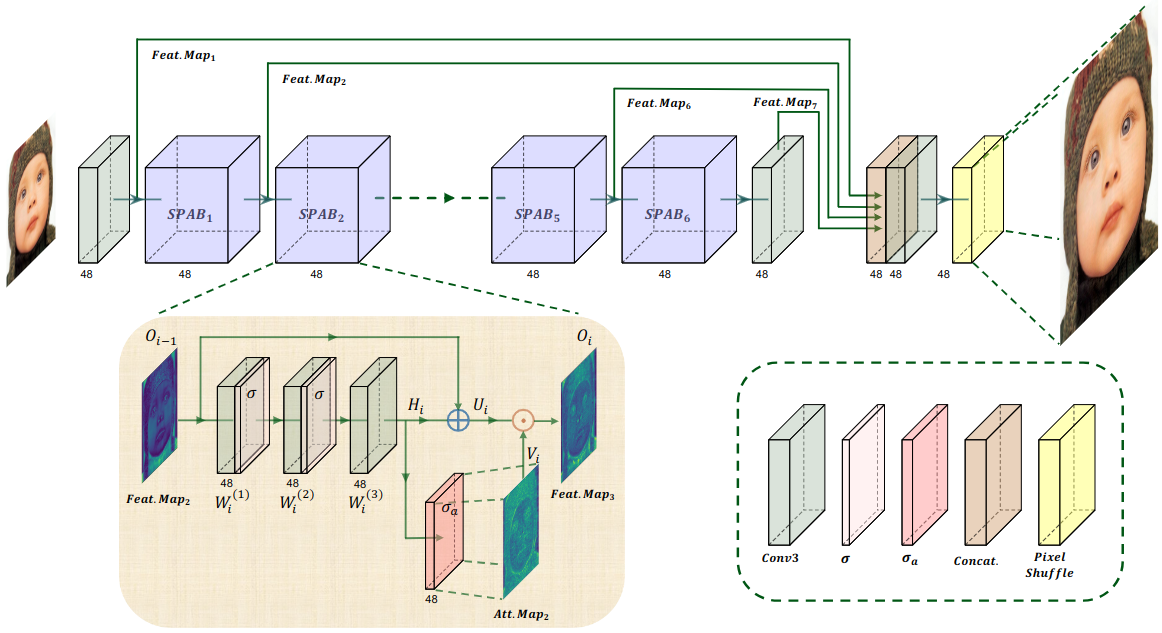
\includegraphics[width=1\linewidth]{images/span.png}
                \caption{Arquitectura del modelo SPAN, que muestra la secuencia de bloques de atención auto-parametrizados (SPAB) y los módulos convolucionales personalizados (\texttt{Conv3XC}) utilizados para extraer características a través de convoluciones y conexiones residuales. La sección ampliada ilustra el flujo interno dentro de un bloque SPAB, donde la atención se genera de forma libre de parámetros mediante funciones de activación simétricas, maximizando la representación de características relevantes sin añadir parámetros adicionales. Este esquema destaca cómo el modelo integra mapas de características y mapas de atención para mejorar la resolución de la imagen de entrada. Recuperado de \textcite{wan2024swiftparameterfreeattentionnetwork}.}
                \label{fig:span}
            \end{figure}


    \subsection{Fusión x2: mejora de resolución intermedia}

        La primera etapa, Fusión x2, se enfoca en duplicar la resolución espacial, permitiendo que las bandas de 20 metros alcancen una resolución de 10 metros. Este proceso sienta las bases para una posterior mejora en la etapa de Fusión x4, unificando la mayoría de las bandas en una resolución común y enriqueciendo la información disponible.

        \subsubsection{Ajustes en la preparación de datos}

            \paragraph{Bandas de 10 metros}

                Estas bandas se redimensionan a una resolución espacial de 20 metros mediante interpolación bilineal con antialiasing. Este ajuste iguala su resolución con las bandas de 20 metros, permitiendo una integración coherente en el modelo y asegurando que los detalles característicos de las bandas de alta resolución se conserven.

            \paragraph{Bandas de 20 metros}

                Inicialmente, se reducen a una resolución de 40 metros utilizando interpolación bilineal con antialiasing. Posteriormente, se reescalan nuevamente a 20 metros aplicando el mismo método. Este proceso de reducción y ampliación facilita que las bandas mantengan coherencia espacial con las bandas de 10 metros ajustadas, preparando los datos para su procesamiento conjunto en el modelo.


        \subsubsection{Componentes}
   
            \paragraph{Entrada}

                Concatenación de las bandas de 10 metros escaladas a 20 metros y las bandas de 20 metros ajustadas. Esta combinación proporciona al modelo una fuente consistente de detalles espaciales y espectrales.

            \paragraph{Objetivo}

                Las bandas originales de 20 metros sirven como referencia para el aprendizaje supervisado, permitiendo al modelo reconstruir los detalles espectrales.

            \paragraph{Salida}

                Una representación fusionada que combina las características espectrales de las bandas de 20 metros con los detalles espaciales de las bandas de referencia, mejorando la resolución y el detalle de la imagen.
        
            \begin{figure}[H] 
                \caption{\doublespacing \\ \textit{Proceso de Fusión x2 en Superresolución}} 
                \centering
                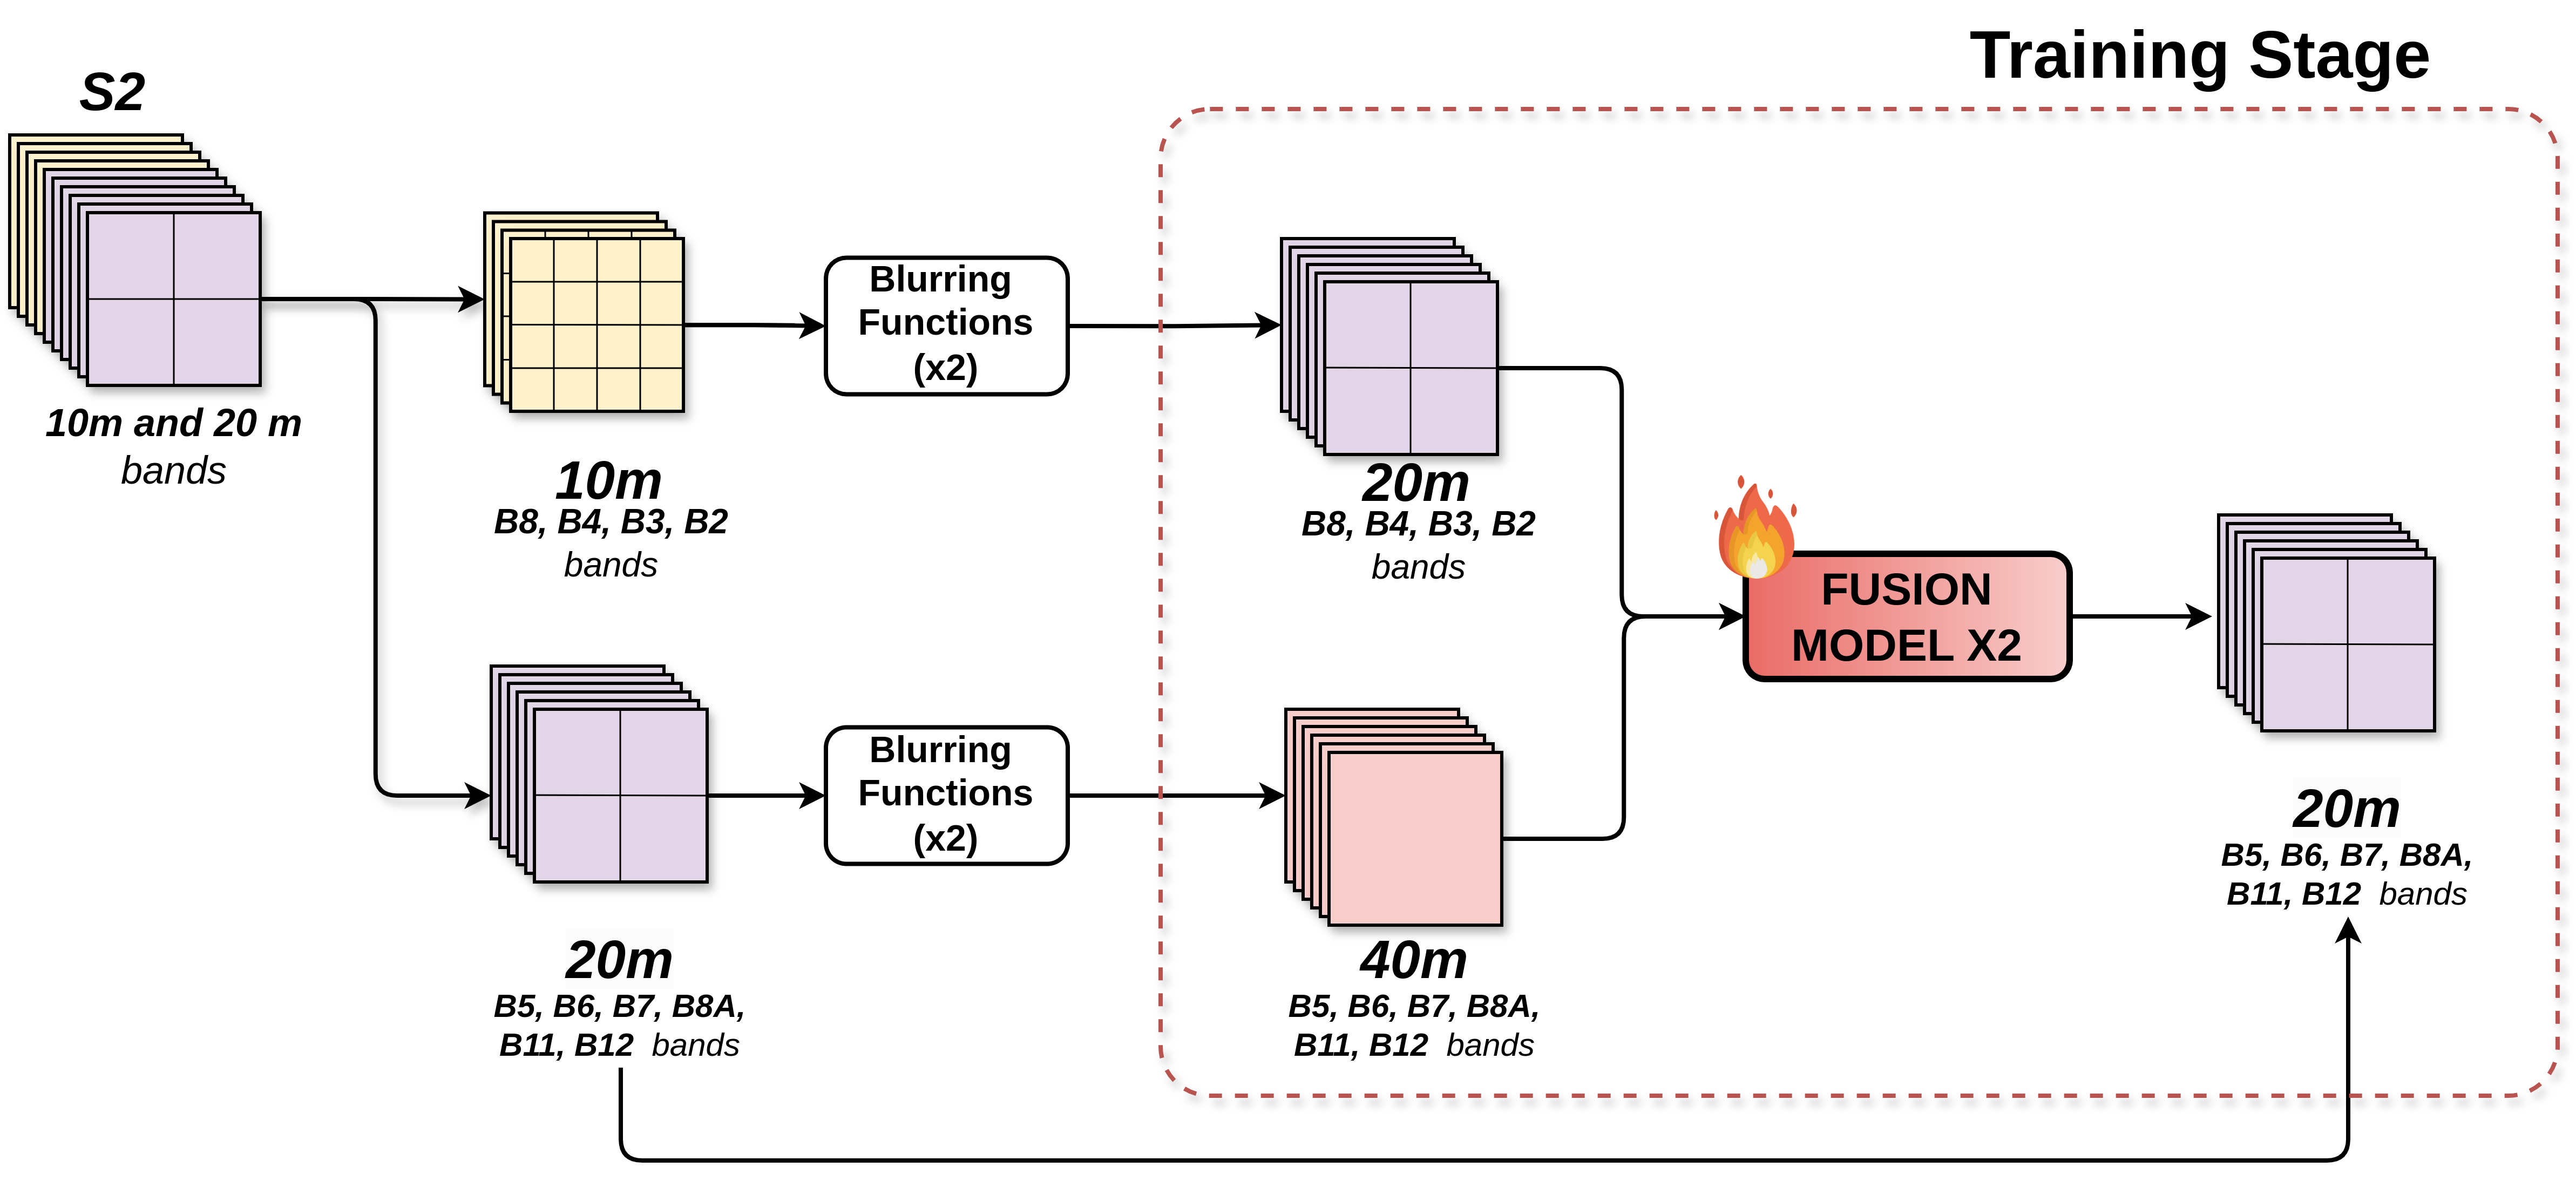
\includegraphics[width=1\linewidth]{images/fusionx2_training.png}
                \begin{justify}
                    \textit{Nota.} Esquema que muestra la preparación de datos y el modelo de Fusión x2, donde las bandas de entrada son ajustadas en resolución para generar una salida unificada de 20 metros, combinando detalles espaciales y espectrales. Elaboración propia.
                \end{justify}                    
                \label{fig:fusionx2_training}
            \end{figure}

        \subsubsection{Filtrado en el dominio de Fourier}

            Se aplica un filtro Butterworth de orden 6 con un factor de escala correspondiente a la duplicación de la resolución. El proceso incluye:

            \begin{itemize}
                \item \textbf{Transformación FFT}: Las imágenes interpoladas y las generadas por el modelo se transforman al dominio de Fourier mediante la Transformada Rápida de Fourier.
                \item \textbf{Aplicación de máscaras de frecuencia}: Se aplica una máscara de paso bajo a la imagen interpolada y una máscara de paso alto complementaria a la imagen de super-resolución, integrando las frecuencias bajas y altas de manera equilibrada.
                \item \textbf{Transformación inversa FFT}: Se realiza la transformación inversa para regresar al dominio espacial, obteniendo una versión filtrada que sirve como salida optimizada del modelo.
            \end{itemize}

            Este filtrado asegura un balance adecuado entre coherencia espacial y detalle, optimizando el rendimiento en la fase de super-resolución.

        \subsubsection{Configuración del modelo}

            El modelo se configura con parámetros específicos para la Fusión x2:

            \begin{itemize}
                \item \textbf{Número de bloques SPAB}: 10 bloques para lograr un equilibrio entre rendimiento y complejidad computacional.
                \item \textbf{Canales de características}: 48 canales para capturar detalles finos en las características de la imagen.
                \item \textbf{Factor de escala}: 2, correspondiente a la duplicación de la resolución espacial.
                \item \textbf{Entradas y salidas}: 10 canales de entrada (bandas ajustadas) y 6 canales de salida (bandas fusionadas).
            \end{itemize}

            Se entrenaron diferentes configuraciones, variando su complejidad y capacidad para evaluar su desempeño. Las configuraciones utilizadas son las siguientes:

            \begin{lstlisting}[language=Python]
                cnn_lightweight = {
                    "in_channels": 10,
                    "out_channels": 6,
                    "feature_channels": 24,
                    "upscale": 1,
                    "bias": True,
                    "train_mode": True,
                    "num_blocks": 6,
                }
                
                cnn_small = {
                    "in_channels": 10,
                    "out_channels": 6,
                    "feature_channels": 48,
                    "upscale": 1,
                    "bias": True,
                    "train_mode": True,
                    "num_blocks": 16,
                }
                
                cnn_medium = {
                    "in_channels": 10,
                    "out_channels": 6,
                    "feature_channels": 72,
                    "upscale": 1,
                    "bias": True,
                    "train_mode": True,
                    "num_blocks": 20
                }
                
                cnn_expanded = {
                    "in_channels": 10,
                    "out_channels": 6,
                    "feature_channels": 96,
                    "upscale": 1,
                    "bias": True,
                    "train_mode": True,
                    "num_blocks": 24,
                }
            \end{lstlisting}


            En estas configuraciones, se varían los parámetros como el número de canales de características (\texttt{feature\_channels}) y el número de bloques SPAB (\texttt{num\_blocks}). El parámetro \texttt{upscale} se establece en 1, ya que en esta implementación el modelo opera en la misma resolución de entrada y salida, enfocándose en mejorar la calidad y detalle de la imagen a través del procesamiento interno del modelo.

            El objetivo de utilizar diferentes tamaños de modelo es evaluar cómo la capacidad del modelo afecta al rendimiento en la tarea de super-resolución. Modelos más pequeños, como el \textit{lightweight}, tienen menos parámetros y requieren menos recursos computacionales, pero pueden tener una capacidad limitada para capturar detalles finos. Por otro lado, modelos más grandes, como el \textit{expanded}, tienen mayor capacidad para aprender representaciones complejas, pero a costa de un mayor tiempo de entrenamiento y requerimientos de hardware.

        \subsubsection{Función de pérdida y entrenamiento}
            \label{sec:funcion_perdida_fusionx2}

            Para el entrenamiento del modelo, se utiliza la función de pérdida L1, que mide la diferencia absoluta media entre la salida del modelo y las bandas originales de 20 metros. Esta función es adecuada para preservar detalles y minimizar artefactos en la imagen resultante, siendo especialmente efectiva en tareas de super-resolución donde la precisión en los valores de los píxeles es crucial.

            % \begin{lstlisting}[language=Python]
            % from loss import l1_loss
            % loss_fn = l1_loss()
            % \end{lstlisting}

            El modelo se entrena utilizando un optimizador AdamW con una tasa de aprendizaje inicial de $1 \times 10^{-4}$ y un decaimiento de peso de $1 \times 10^{-2}$, lo que ayuda a prevenir el sobreajuste y a mejorar la generalización del modelo. Además, se emplea un programador de tasa de aprendizaje cíclico (\texttt{CyclicLR}) para ajustar dinámicamente la tasa de aprendizaje durante el entrenamiento, favoreciendo una convergencia más rápida y estable.

            \begin{lstlisting}[language=Python]
            optimizer = torch.optim.AdamW(
                            self.parameters(), 
                            lr=self.learning_rate, 
                            weight_decay=1e-2)
            scheduler = torch.optim.lr_scheduler.CyclicLR(
                            optimizer, 
                            base_lr=1e-5, 
                            max_lr=1e-3, 
                            step_size_up=1000)
            \end{lstlisting}

            El entrenamiento se realiza con un tamaño de lote de 4 y durante 50 épocas. Se aplica una estrategia de parada temprana (\textit{early stopping}) basada en la pérdida de validación para evitar el sobreentrenamiento. Estas configuraciones permiten al modelo aprender de manera eficiente y efectiva, logrando una reducción significativa en la pérdida y mejorando la calidad de las imágenes de super-resolución generadas.


            \begin{figure}[H]
                \centering
                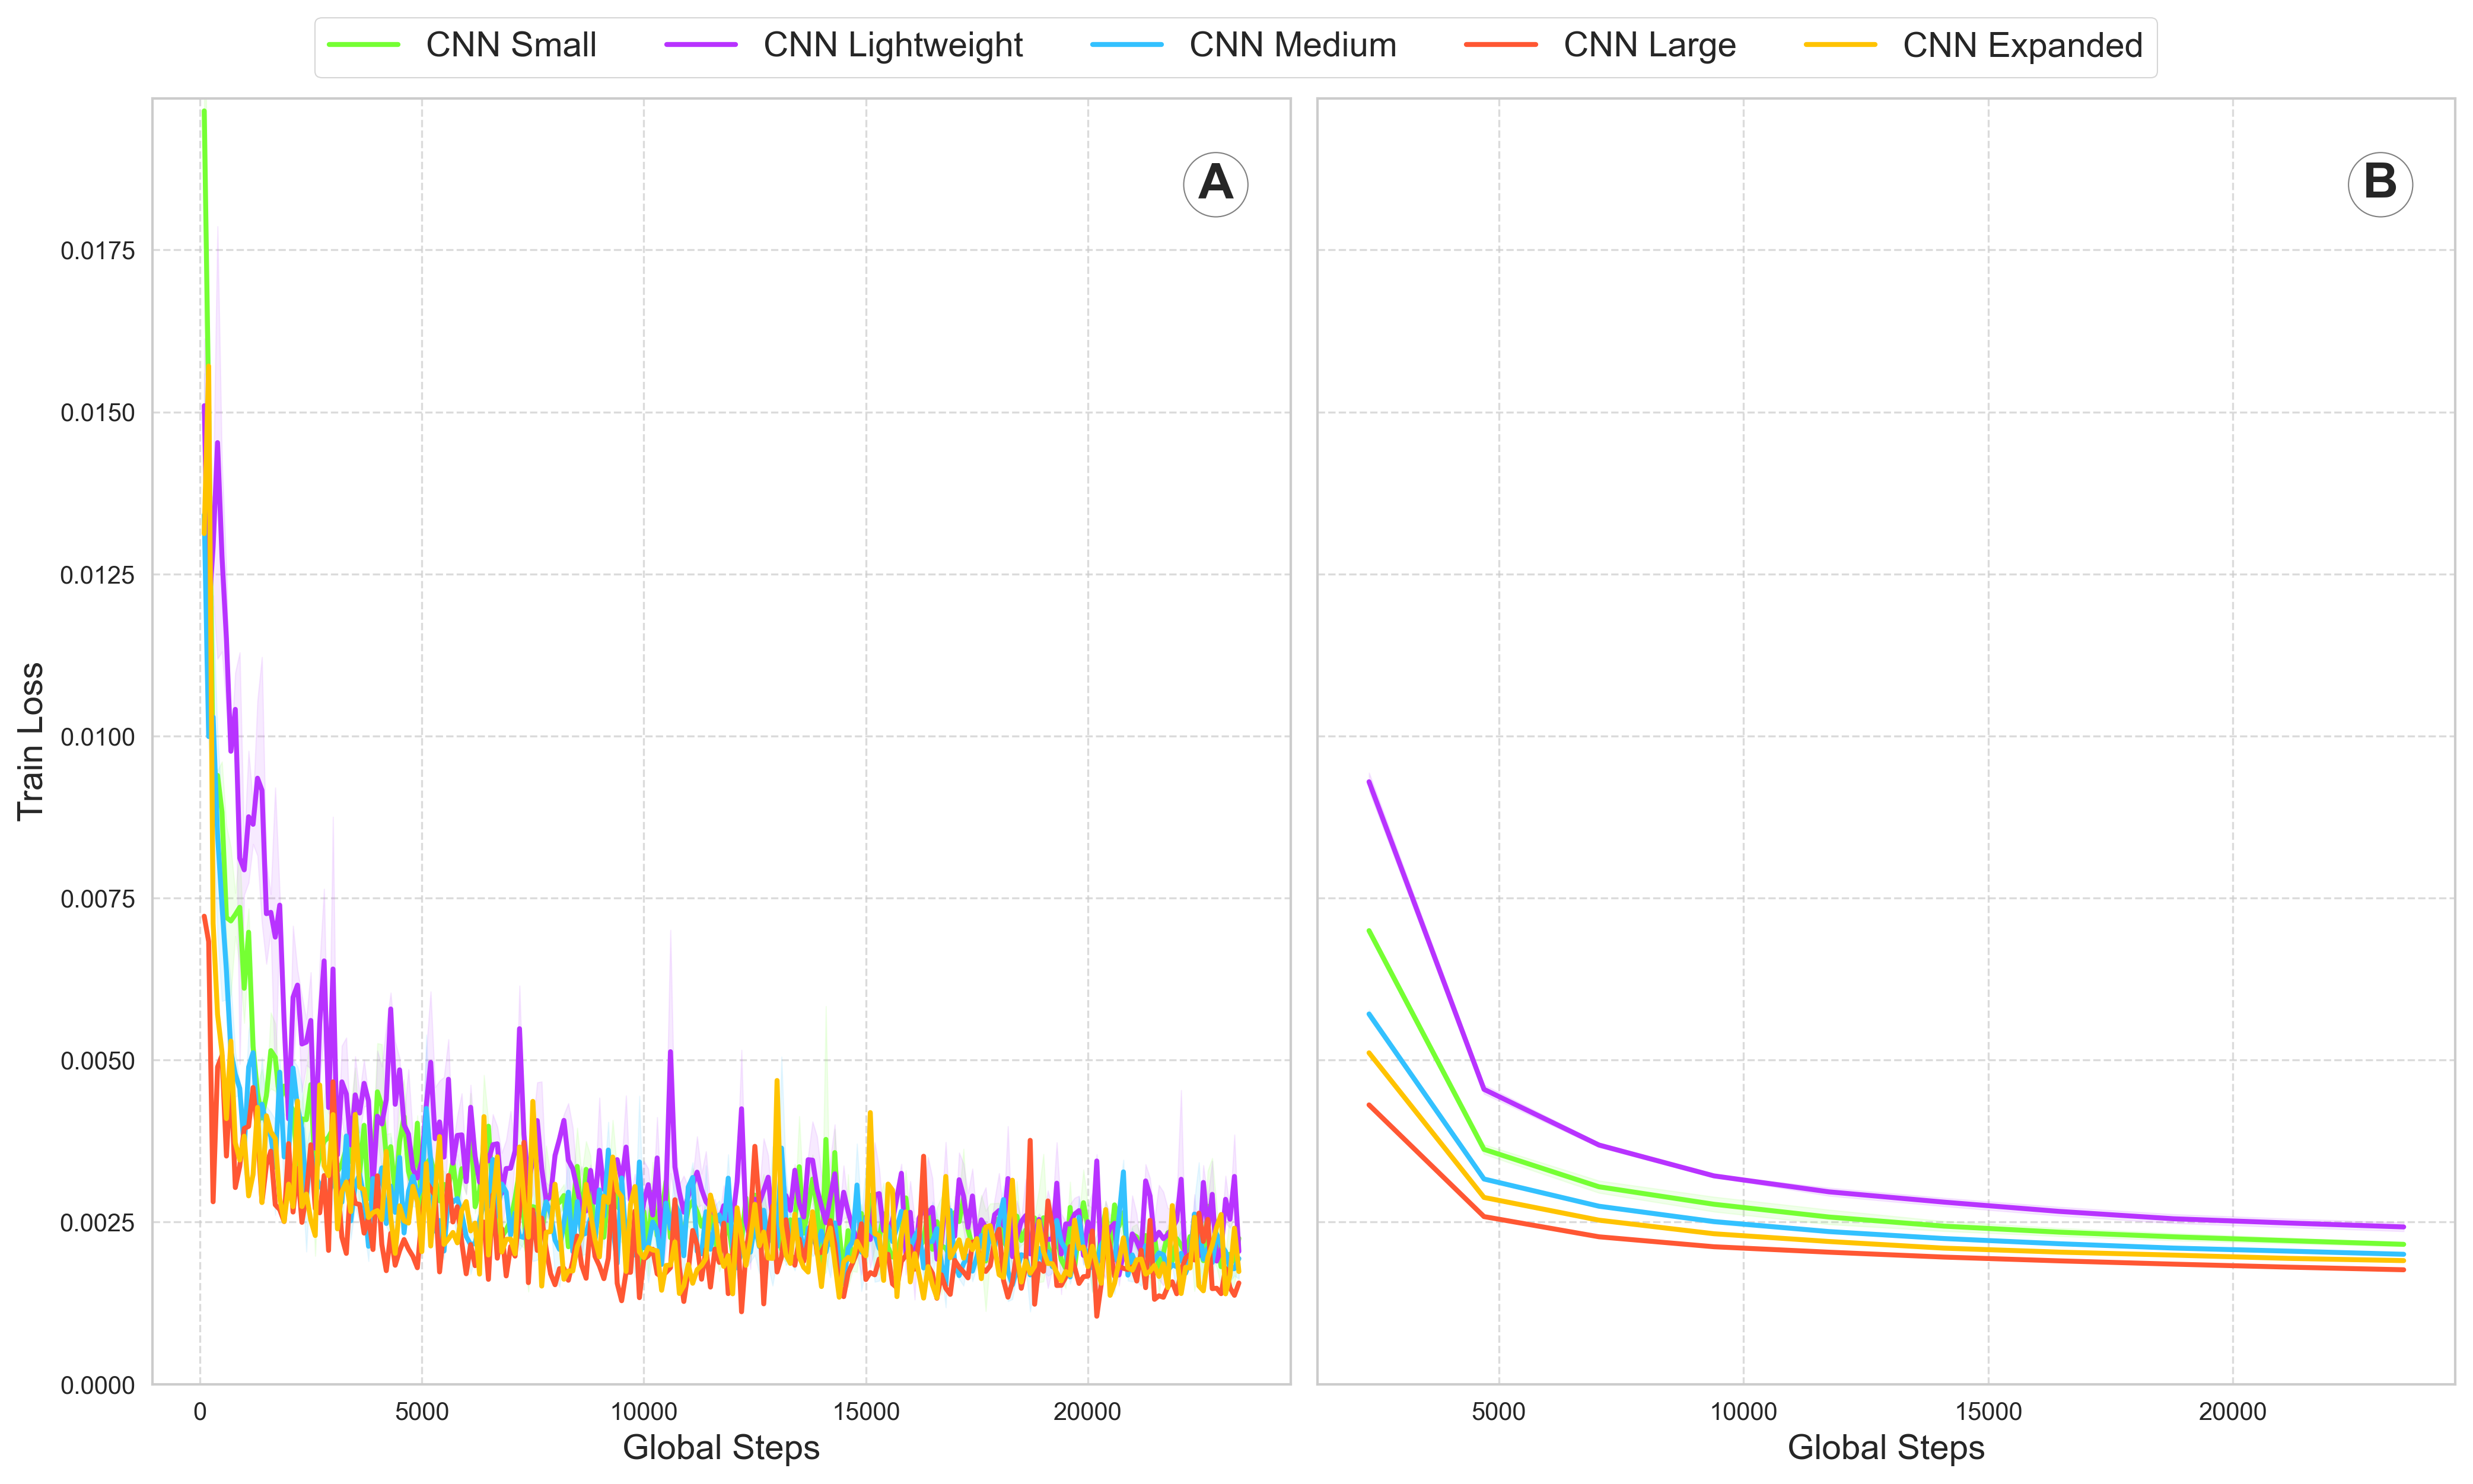
\includegraphics[width=1\linewidth]{images/loss_train_fusionx2.png}
                \caption{Comparación de la pérdida de entrenamiento para distintas configuraciones del modelo de fusión en super-resolución. En el panel A (izquierda), se observa la pérdida en función de los pasos globales, mostrando la estabilidad de cada configuración a lo largo del entrenamiento. En el panel B (derecha), la pérdida se presenta por épocas, donde las arquitecturas más complejas (Medium, Expanded, Large) convergen más rápidamente y logran menores valores de pérdida, lo que sugiere una mayor capacidad para capturar detalles en la tarea de super-resolución.}


                \label{fig:loss_train_fusionx2}
            \end{figure}


    \subsection{Fusión x4: mejora de resolución a nivel fino}

        La segunda etapa, Fusión x4, se enfoca en cuadruplicar la resolución espacial, obteniendo imágenes de 10 metros a partir de bandas originalmente de 40 metros. Esta fase aprovecha los resultados de la Fusión x2 para alcanzar una mayor fidelidad y detalle en la imagen final.

        \subsubsection{Ajustes en la preparación de datos}

            \paragraph{Bandas de 10 metros}

                Se utilizan sin cambios, proporcionando detalles espaciales críticos que enriquecen la entrada del modelo.

            \paragraph{Bandas de 20 metros}

                Se someten al siguiente proceso:

                \begin{itemize}
                    \item \textbf{Reducción a 40 metros}: Se reducen a una resolución de 40 metros mediante interpolación bilineal con antialiasing.
                    \item \textbf{Ampliación a 10 metros}: Posteriormente, se reescalan a una resolución de 10 metros utilizando el mismo método, permitiendo su integración con las bandas de 10 metros originales.
                \end{itemize}

            \paragraph{Bandas de 40 metros}

                Las bandas ajustadas a 40 metros se interpolan directamente a 10 metros mediante interpolación bilineal con antialiasing, proporcionando una representación adicional que enriquece la información espectral.

        \subsubsection{Definición de entrada, objetivo y salida}

            \begin{itemize}
                \item \textbf{Entrada}: Concatenación de las bandas de 40 metros interpoladas a 10 metros y las bandas de 10 metros originales, resultando en 10 canales de entrada.
                \item \textbf{Objetivo}: La salida generada por el modelo de Fusión x2 aplicado a las bandas de 20 metros, proporcionando una referencia refinada para el aprendizaje.
                \item \textbf{Salida}: Una imagen de super-resolución que combina efectivamente las características espectrales y espaciales, alcanzando una resolución de 10 metros con detalles refinados.
            \end{itemize}

        \subsubsection{Filtrado en el dominio de Fourier}

            Se utiliza un filtro Butterworth de orden 6 ajustado para reflejar el factor de escala de 4. El proceso sigue los mismos pasos descritos anteriormente, adaptándose al nuevo factor de escala.


        \subsubsection{Configuración del modelo}

            Para la Fusión x4, se entrenan diferentes configuraciones del modelo CNNSR con el objetivo de evaluar su rendimiento y determinar la arquitectura más adecuada para la tarea. Estas configuraciones varían en términos de complejidad y capacidad, ajustando parámetros clave como el número de bloques SPAB y los canales de características.

            Para la Fusión x4, se realizan ajustes específicos en el modelo:

            \begin{itemize}
                \item \textbf{Número de bloques SPAB}: 20 bloques para capturar detalles más finos y profundizar el aprendizaje.
                \item \textbf{Canales de características}: 72 canales para manejar la complejidad adicional de la tarea.
                \item \textbf{Factor de escala}: 1 (la salida es de la misma resolución que la entrada, pero con mayor detalle).
                \item \textbf{Entradas y salidas}: 10 canales de entrada y 6 canales de salida.
            \end{itemize}

            Se entrenaron diferentes configuraciones, variando su complejidad y capacidad para evaluar su desempeño. Las configuraciones utilizadas son las siguientes:

            \begin{lstlisting}[language=Python]
            cnn_lightweight = {
                "in_channels": 10,
                "out_channels": 6,
                "feature_channels": 24,
                "upscale": 1,
                "bias": True,
                "train_mode": True,
                "num_blocks": 6,
            }

            cnn_small = {
                "in_channels": 10,
                "out_channels": 6,
                "feature_channels": 48,
                "upscale": 1,
                "bias": True,
                "train_mode": True,
                "num_blocks": 16,
            }

            cnn_medium = {
                "in_channels": 10,
                "out_channels": 6,
                "feature_channels": 72,
                "upscale": 1,
                "bias": True,
                "train_mode": True,
                "num_blocks": 20,
            }

            cnn_expanded = {
                "in_channels": 10,
                "out_channels": 6,
                "feature_channels": 96,
                "upscale": 1,
                "bias": True,
                "train_mode": True,
                "num_blocks": 24,
            }

            cnn_large = {
                "in_channels": 10,
                "out_channels": 6,
                "feature_channels": 150,
                "upscale": 1,
                "bias": True,
                "train_mode": True,
                "num_blocks": 36,
            }
            \end{lstlisting}

            Estas configuraciones permiten explorar cómo la complejidad del modelo afecta el rendimiento en la tarea de Fusión x4, desde modelos más ligeros hasta arquitecturas más profundas y con mayor capacidad de representación. Al evaluar estas variantes, es posible identificar un equilibrio óptimo entre el rendimiento y los recursos computacionales requeridos.

        \subsubsection{Integración con el modelo de Fusión x2}

            El modelo de Fusión x2 se utiliza para generar el objetivo que servirá como referencia en el entrenamiento de Fusión x4. Se cargan los pesos del modelo de Fusión x2 y se congela su entrenamiento:

            \begin{lstlisting}[language=Python]
                # Cargar el modelo de Fusión x2
                weights = torch.load(fusion_model, map_location="cpu")
                fusionx2_model = utils.load_model(model_name="cnn", model_size="medium")
                fusionx2_model.load_state_dict(weights)
                fusionx2_model.eval()
                for param in fusionx2_model.parameters():
                    param.requires_grad = False
            \end{lstlisting}

            \begin{figure}[H]
                \centering
                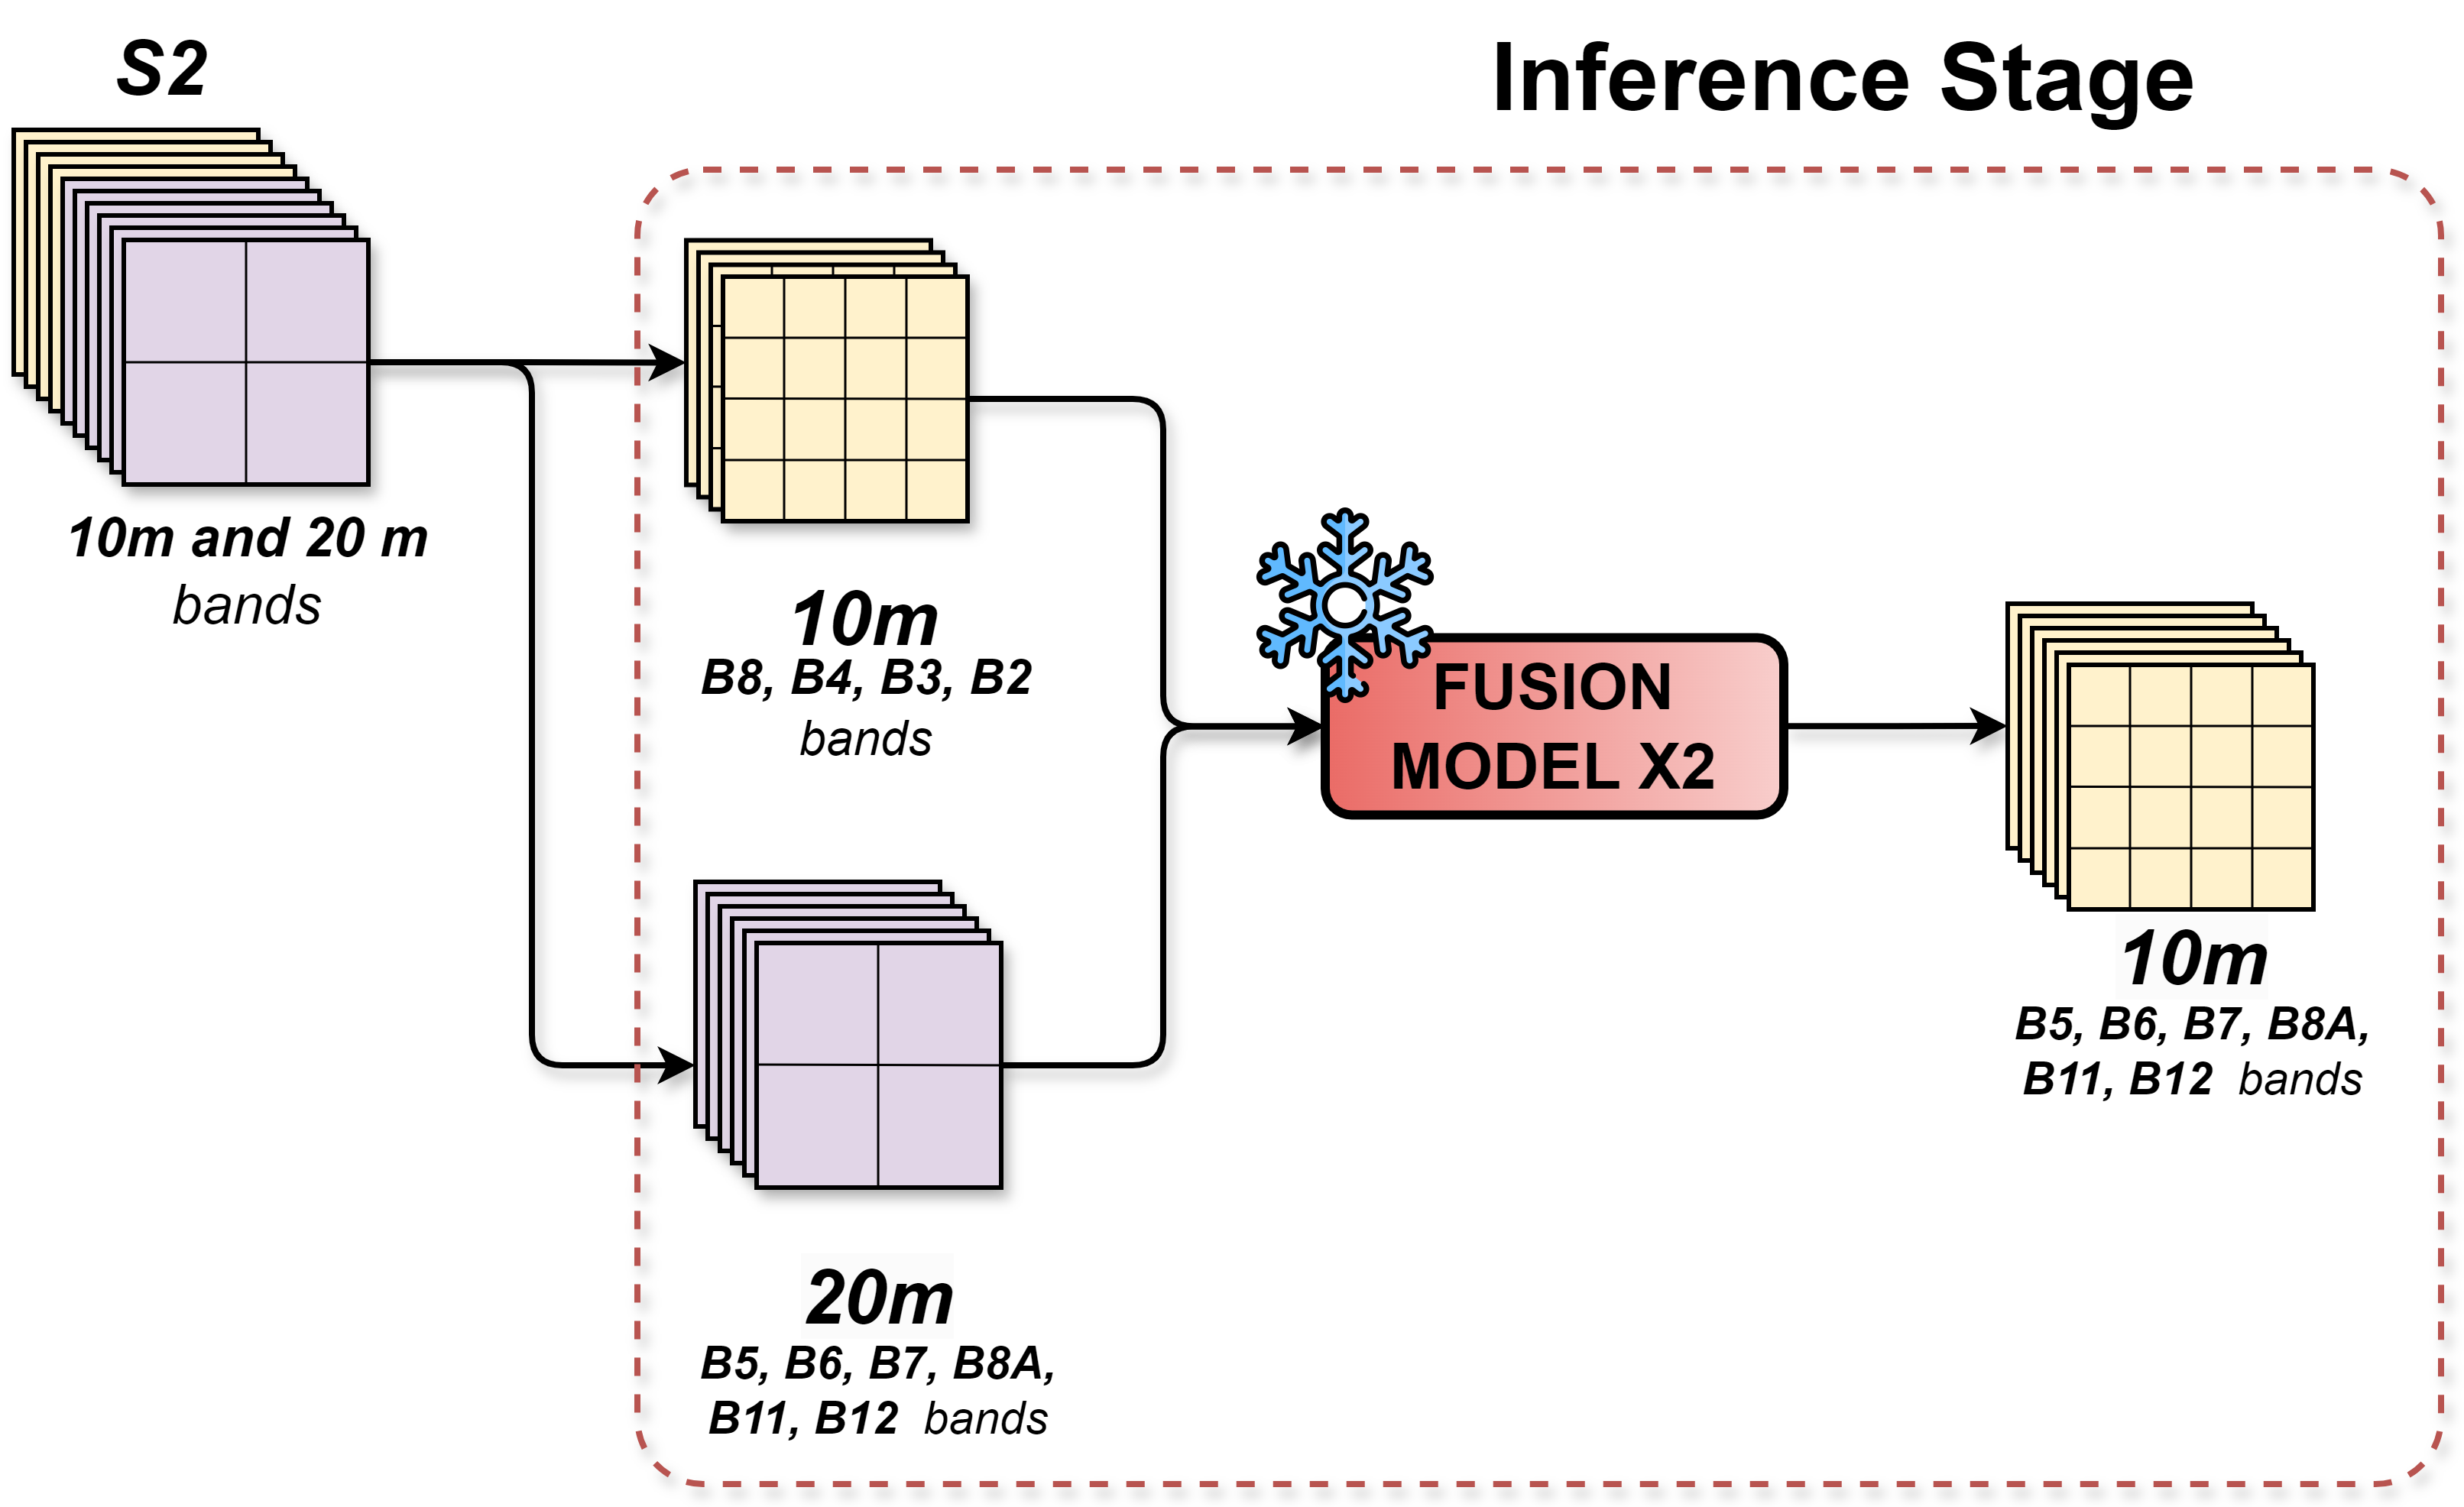
\includegraphics[width=0.65\linewidth]{images/inference_fusionx2.png}
                    \caption{Diagrama del proceso de Fusión x2 en super-resolución. Las bandas de entrada a 20 metros y las de mayor resolución, preprocesadas con funciones de desenfoque, se integran en el modelo de Fusión x2. Este modelo produce una salida de 10 metros de resolución, combinando la información espacial de las bandas de alta resolución con la riqueza espectral de las de menor resolución. Este paso intermedio sirve para unificar las bandas en una resolución común y optimizar la información para la etapa de Fusión x4.}

                \label{fig:fusionx4_training}
            \end{figure}


        \subsubsection{Implementación del filtrado con \textit{Hard Constraint}}

            Se utiliza un \textit{Hard Constraint} basado en una capa convolucional con pesos predefinidos que implementa el filtro Butterworth de orden 6. Esto asegura que los componentes de baja frecuencia de la imagen interpolada se mantengan durante el procesamiento:

            \begin{lstlisting}[language=Python]
            self.hard_constraint = CNNHardConstraint(
                filter_method="butterworth",
                filter_hyperparameters={"order": 6},
                scale_factor=2,
                in_channels=6,
                out_channels=[0, 1, 2, 3, 4, 5],
                device=device,
            )
            \end{lstlisting}

            \begin{figure}[H]
                \centering
                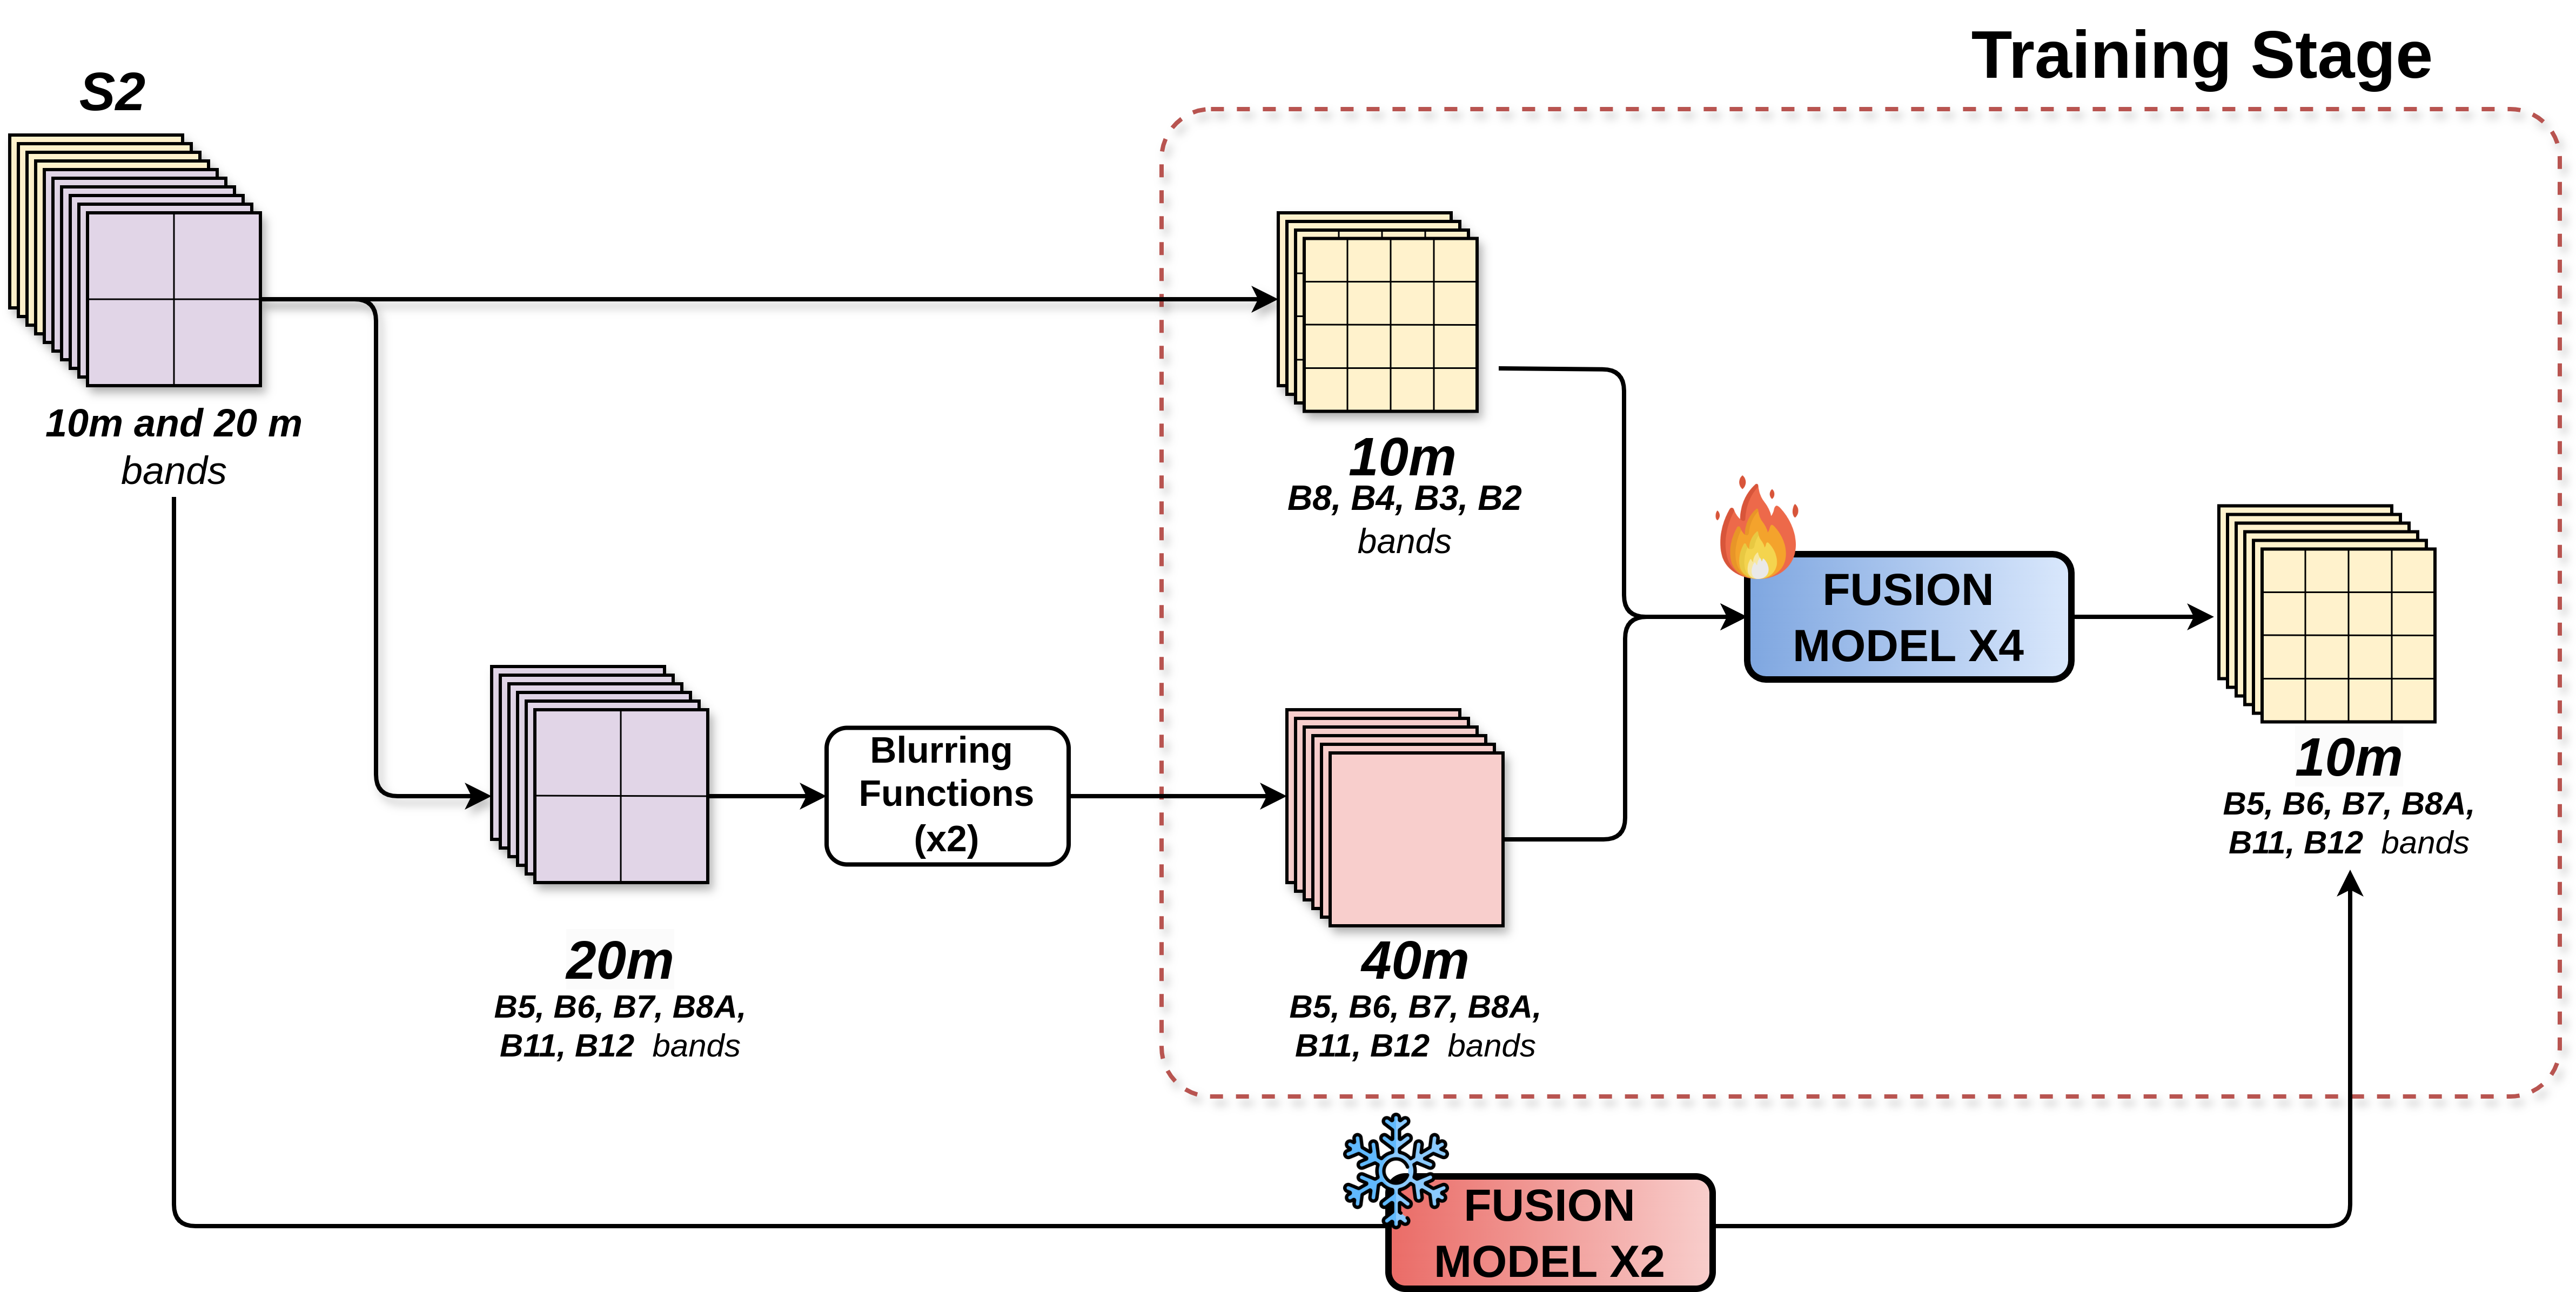
\includegraphics[width=1\linewidth]{images/fusionx4_training.png}
                \caption{Diagrama del proceso de Fusión x4 en super-resolución. Se muestra la preparación de datos, en la que se aplican funciones de desenfoque (\textit{Blurring Functions}) para reducir la resolución inicial de las bandas. Las bandas de 20 metros y las de mayor resolución (preprocesadas por el modelo de Fusión x2) son combinadas mediante el modelo de Fusión x4, que genera una salida final de 10 metros de resolución. Este modelo permite aumentar la fidelidad espacial de las bandas, integrando información de diferentes resoluciones para obtener una imagen más detallada y precisa.}
                \label{fig:fusionx4_training}
            \end{figure}

        \subsubsection{Función de pérdida y entrenamiento}

            Para el entrenamiento del modelo de Fusión x4, se utiliza la \textit{superloss}, una combinación de funciones de pérdida que incluye L1, LPIPS y CLIP. Esta función permite al modelo aprender no solo diferencias pixel a pixel, sino también características perceptuales y semánticas de alto nivel, mejorando la calidad visual y la coherencia del contenido en la imagen resultante.

            Los componentes de la \textit{superloss} son:

            \begin{itemize}
                \item \textbf{L1 Loss} ($L_{\text{L1}}$): Calcula la diferencia absoluta media entre los píxeles de la imagen generada y la imagen objetivo, enfocándose en la precisión de bajo nivel.
                \item \textbf{LPIPS Loss} ($L_{\text{LPIPS}}$): Evalúa la similitud perceptual entre las imágenes utilizando características de redes neuronales profundas, capturando la calidad visual desde una perspectiva humana.
                \item \textbf{CLIP Loss} ($L_{\text{CLIP}}$): Utiliza el modelo CLIP para comparar características semánticas de alto nivel, asegurando que la imagen generada mantenga coherencia en términos de contenido.
            \end{itemize}

            La función de pérdida total se define como:

            \[
            \text{SuperLoss} = \lambda_1 \cdot L_{\text{L1}} + \lambda_2 \cdot L_{\text{LPIPS}} + \lambda_3 \cdot L_{\text{CLIP}}
            \]

            Donde los pesos $\lambda_1 = 17.7474$, $\lambda_2 = 0.8778$ y $\lambda_3 = 2.4049$ se establecen para equilibrar la contribución de cada término.

            % \begin{lstlisting}[language=Python]
            % from loss import super_loss
            % loss_fn = super_loss(device=device)
            % \end{lstlisting}

            El modelo se entrena utilizando PyTorch Lightning, con el mismo optimizador AdamW y programador de tasa de aprendizaje cíclico (\texttt{CyclicLR}) descritos en la sección de Fusión x2 (ver Sección \ref{sec:funcion_perdida_fusionx2}). Esto asegura una convergencia efectiva y un desempeño óptimo del modelo. Se utiliza una tasa de aprendizaje inicial de $1 \times 10^{-4}$ y un tamaño de lote de 4, entrenando el modelo durante 50 épocas. Al igual que en Fusión x2, se implementa una estrategia de parada temprana basada en la pérdida de validación para evitar el sobreentrenamiento.

            \begin{figure}[H]
                \centering
                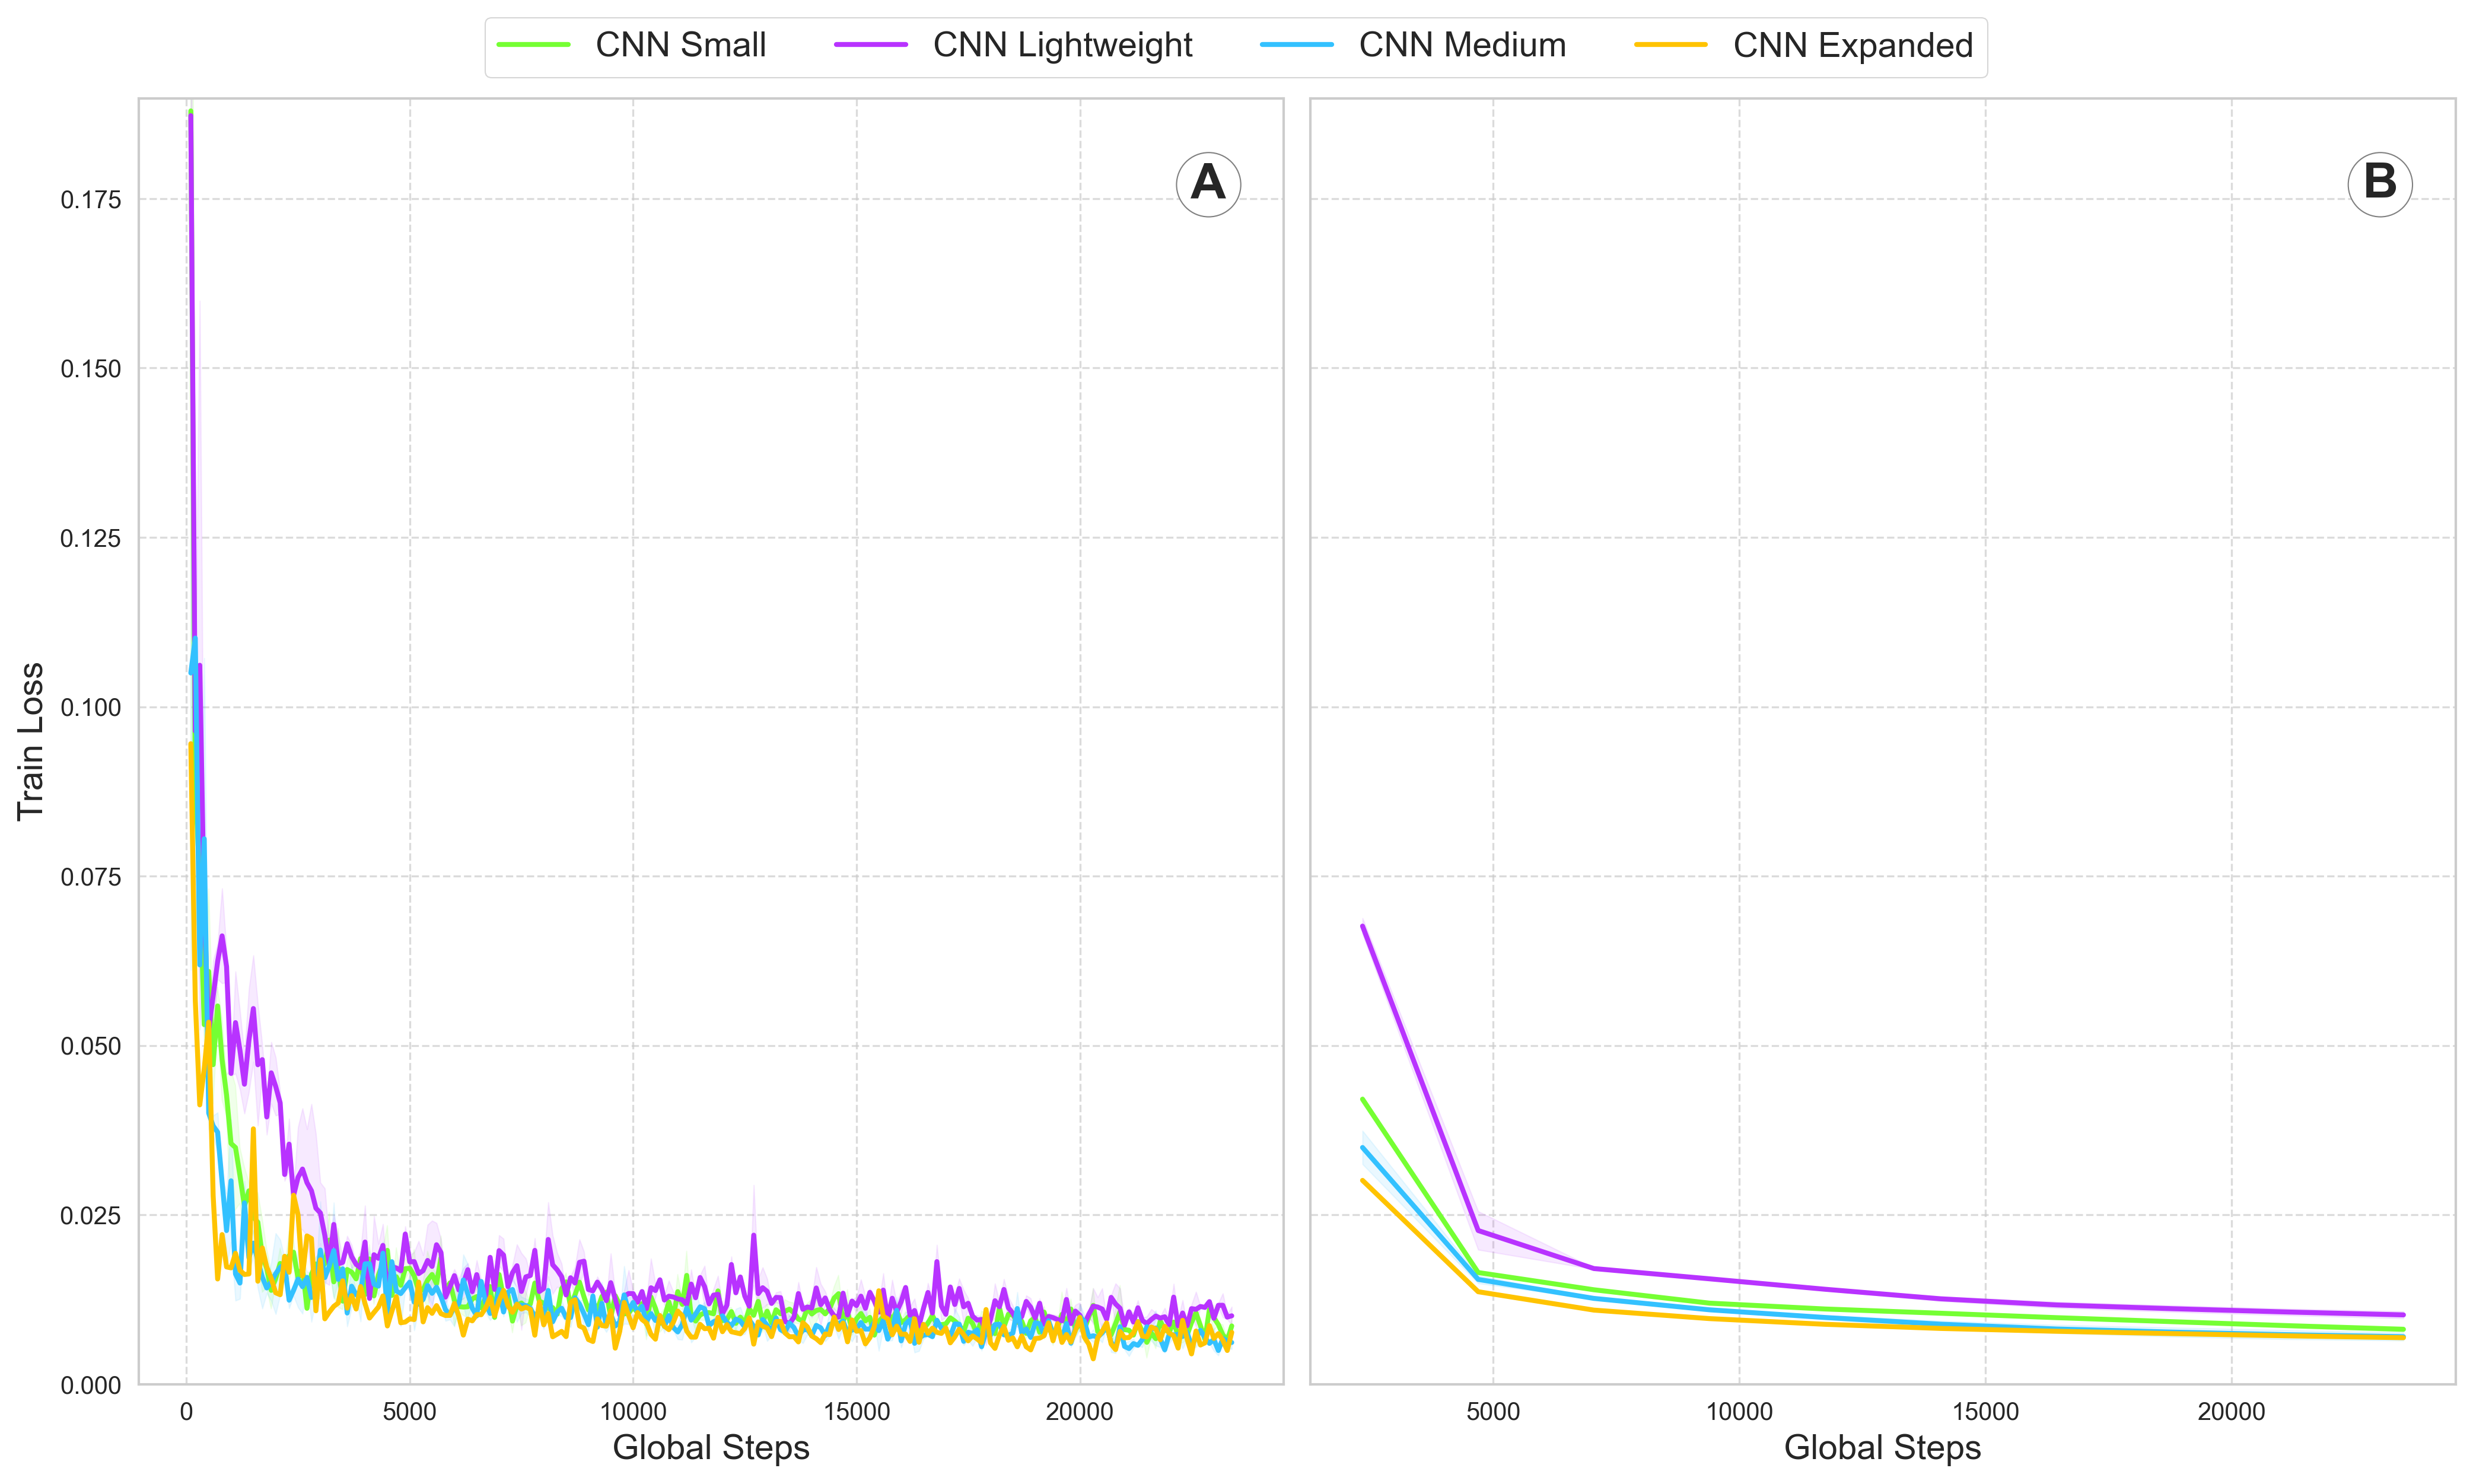
\includegraphics[width=1\linewidth]{images/loss_train_fusionx4.png}
                \caption{Evolución de la pérdida de entrenamiento durante el entrenamiento del modelo de Fusión x4 para diferentes configuraciones de CNN. En el panel A (izquierda), la pérdida se representa en función de los pasos globales, mostrando la estabilidad y comportamiento de cada configuración a medida que avanza el entrenamiento. En el panel B (derecha), se observa la pérdida suavizada, destacando la convergencia de cada arquitectura hacia menores valores de pérdida. Las arquitecturas más complejas, como CNN Expanded, logran menores pérdidas finales, indicando una mayor capacidad para capturar detalles en la super-resolución.}
                \label{fig:loss_train_fusionx4}
            \end{figure}

        \subsubsection{Análisis de la pérdida de testeo}

            Además de evaluar la pérdida durante el entrenamiento, es fundamental analizar el desempeño del modelo en el conjunto de testeo para validar su capacidad de generalización y asegurar que no se esté sobreajustando a los datos de entrenamiento. La Figura~\ref{fig:test_loss_comparison} presenta una comparación de la pérdida de testeo para las diferentes configuraciones del modelo CNN en las etapas de Fusión x2 y Fusión x4.

            \begin{figure}[H]
                \centering
                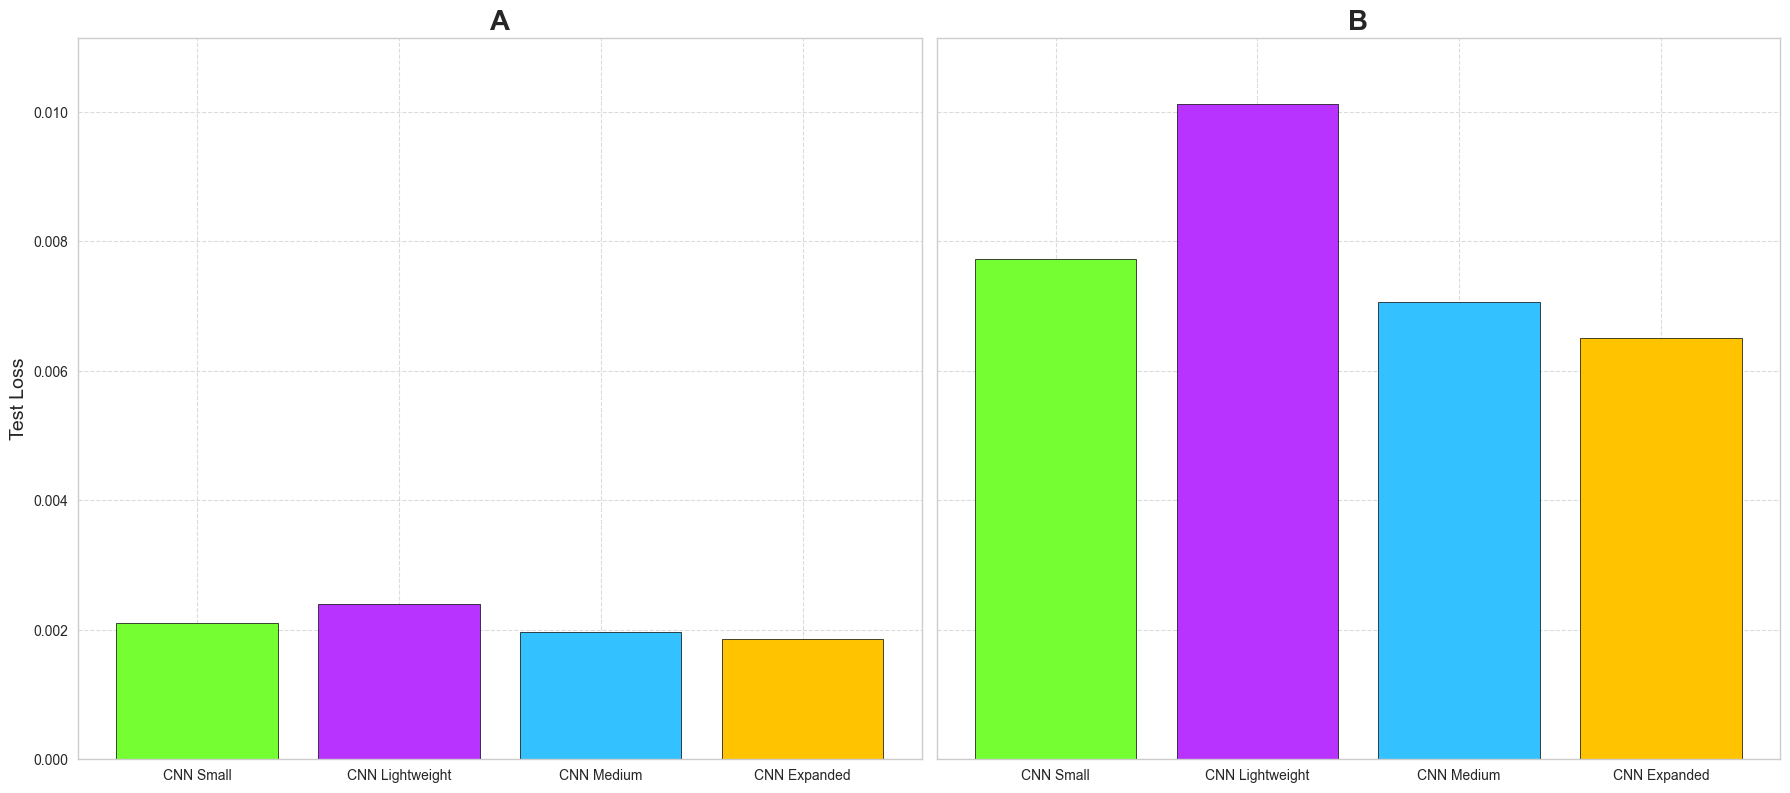
\includegraphics[width=1\linewidth]{images/fusionx2x4_loss_test.png}
                \caption{Comparación de la pérdida de testeo para distintas configuraciones de CNN en las etapas de Fusión x2 y Fusión x4. En el panel A (izquierda), se observa la pérdida de testeo para la Fusión x2, con resultados relativamente homogéneos entre arquitecturas, pero con una ligera ventaja en las configuraciones de mayor capacidad. En el panel B (derecha), correspondiente a la Fusión x4, se evidencia una mayor variabilidad, donde las arquitecturas más complejas, como CNN Expanded, logran menores pérdidas, indicando un rendimiento superior en la resolución final de 10 metros.}
                \label{fig:fusionx2x4_loss_test}
            \end{figure}

            En la Figura~\ref{fig:fusionx2x4_loss_test}, se aprecia que, especialmente en la etapa de Fusión x4, las arquitecturas con mayor capacidad tienden a lograr menores valores de pérdida en el conjunto de testeo, sugiriendo una mejor representación y captura de detalles. Sin embargo, los modelos de mayor tamaño también demandan más recursos computacionales y tiempo de entrenamiento, por lo que es necesario equilibrar el rendimiento y la eficiencia según las necesidades y limitaciones específicas de la aplicación.

        \subsubsection{Optimización de la inferencia mediante combinación de convoluciones}

            Durante la etapa de inferencia en Fusión x2, es esencial que el modelo CNNSR sea eficiente, especialmente en entornos con limitaciones de recursos. Para lograr una inferencia rápida sin comprometer la calidad, se ha implementado una optimización que reduce la complejidad computacional al combinar múltiples convoluciones en una sola operación.

            \paragraph{Combinación de convoluciones en \texttt{Conv3XC}}

                El modelo utiliza bloques convolucionales \texttt{Conv3XC}, que durante el entrenamiento aplican tres convoluciones para aprender representaciones complejas de las imágenes:

                \begin{enumerate}
                    \item \textbf{Primera convolución} (\texttt{conv[0]}): Convierte las características de entrada a un espacio intermedio.
                    \item \textbf{Segunda convolución} (\texttt{conv[1]}): Aplica una convolución 3x3 para capturar patrones locales.
                    \item \textbf{Tercera convolución} (\texttt{conv[2]}): Reduce la dimensionalidad a los canales de salida deseados.
                \end{enumerate}

                Además, una conexión residual (\texttt{sk}) conecta la entrada con la salida del bloque mediante una convolución 1x1.

            \paragraph{Optimización en inferencia}

                Para acelerar la inferencia, se combinan las tres convoluciones y la conexión residual en una sola operación mediante:

                \begin{itemize}
                    \item \textbf{Precomputación de pesos y sesgos combinados}: Antes de la inferencia, se combinan los pesos y sesgos de las capas convolucionales en una única convolución.
                    \item \textbf{Uso de una sola convolución en inferencia}: La operación combinada permite reducir el tiempo de procesamiento sin modificar la salida.
                \end{itemize}

                Esta optimización se realiza con la función \texttt{update\_params()} dentro de la clase \texttt{Conv3XC}:

                \begin{lstlisting}[language=Python]
                class Conv3XC(nn.Module):
                    def __init__(...):
                        # Inicialización de capas y variables
                    def update_params(self):
                        # Combina las convoluciones en una operación única
                    def forward(self, x: torch.Tensor) -> torch.Tensor:
                        if self.train_mode:
                            # Durante entrenamiento, usa las convoluciones originales
                            out = self.conv(x) + self.sk(x)
                        else:
                            # En inferencia, usa la convolución combinada
                            self.update_params()
                            out = self.eval_conv(x)
                        return out
                \end{lstlisting}

                Para activar esta optimización:

                \begin{lstlisting}[language=Python]
                # Configurar el modelo para inferencia
                model.train_mode = False
                model.eval()
                with torch.no_grad():
                    output = model(input_data)
                \end{lstlisting}

            \paragraph{Beneficios de la optimización}

                \begin{itemize}
                    \item \textbf{Eficiencia}: Reduce el tiempo de inferencia y uso de recursos.
                    \item \textbf{Escalabilidad}: Permite procesar imágenes de mayor resolución sin aumentar significativamente el tiempo.
                    \item \textbf{Calidad mantenida}: La salida es idéntica a la obtenida sin la optimización.
                \end{itemize}

                Esta técnica es ideal para aplicaciones que requieren procesamiento rápido de grandes volúmenes de datos en tiempo real o cercano al tiempo real.

            \paragraph{Implementación práctica}

                Durante la inferencia en Fusión x2, el modelo utiliza la convolución combinada:

                \begin{lstlisting}[language=Python]
                # Preparar el modelo para la inferencia
                fusionx2_model.train_mode = False
                fusionx2_model.eval()
                # Procesar las imágenes de entrada
                with torch.no_grad():
                    output = fusionx2_model(input_images)
                \end{lstlisting}

                Esta optimización reduce el tiempo de procesamiento sin afectar la calidad de las imágenes generadas.
